\chapter{Digital Communications}

The expression \emph{digital communications} broadly refers to the transmission of information using digital messages or bit streams.
There are notable advantages to transmitting data  using discrete messages.
It allows for enhanced signal processing and quality control.
In particular, errors caused by noise and interference can be detected and corrected.
Digital communications also make the networking of heterogeneous systems possible, with the Internet being the most obvious such example.
These advantages, and many more, explain the widespread adoption and constantly increasing popularity of digital communication systems.


\section{System Components}

A typical digital communication system can be represented by the functional block diagram depicted in Fig~\ref{figure:BlockDiagram}.
It is composed of five basic components.
The input block contains the source, which produces data (such as voice, emails, or images), and it also includes all the operations that are required to convert the original information into a format suitable for transmission.
The transmitter takes bits from the input block and sends them over a channel using electromagnetic signals, or some alternate means.
Communication channels come in many flavors.
For instance, a transmission can take place over an ethernet cable, a coaxial cable, or free space (wireless communications).
There are also more esoteric channels like a hard drive platter, a compact disc, or a memory stick.
The role of the receiver is to recover the sent message from a collection of measurements.
This unit may need to extract the signal from noise and, possibly, correct errors that may have occurred during transmission.
Finally, the output block takes the received information and puts it back in a format that is appropriate for the end-users.

\begin{figure}[htbp]
\begin{center}
\begin{psfrags}
\psfrag{I}[c]{Input}
\psfrag{O}[c]{Output}
\psfrag{T}[c]{Transmitter}
\psfrag{R}[c]{Receiver}
\psfrag{C}[c]{Channel}
\epsfig{file=Figures/diagram,width=10.575cm}
\end{psfrags}
\end{center}
\caption{Block diagram of a digital communication system.}
\label{figure:BlockDiagram}
\end{figure}

Fig.~\ref{figure:BlockDiagram} also allude to the natural symmetry present in digital communication systems.
Operations that take place on the transmitter side must often be undone on the receiver side.
As such, complementary steps are frequently studied in pairs.
Our treatment of digital communications will follow this general approach.


\subsection{The Input-Output Blocks}

The role of the input block is to take information in its natural form and to convert it into a digital format.
Depending on the nature of the source, two operations may be necessary to digitalize a message.
\emph{Sampling} is a signal processing technique that reduces a continuous-time signal to a discrete-time signal.
The conversion of a sound wave into a sequence of samples is a common example of sampling.
The second action that may be required is \emph{quantization}, which maps a continuous-space signal into a discrete set of possible values.
The combination of these two operations will transform a continuous signal into a digital message.

\begin{figure}[htbp]
\begin{center}
\begin{psfrags}
\psfrag{I}[c]{Input}
\psfrag{S}[c]{Sampling}
\psfrag{Q}[c]{Quantization}
\psfrag{E}[c]{Compression}
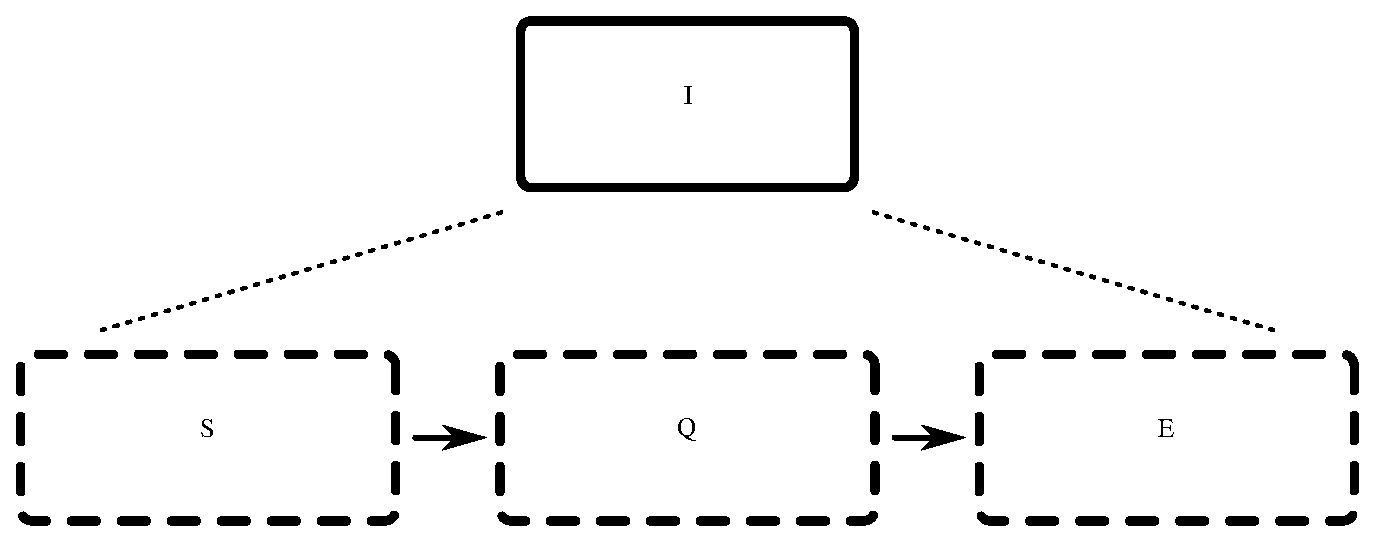
\epsfig{file=Figures/input,width=12.075cm}
\end{psfrags}
\end{center}
\caption{Components of the input block.}
\label{figure:BlockInput}
\end{figure}

The optional step of \emph{data compression}, or source coding, is often used at the input to reduce the size of the message to be transmitted.
This, in turn, brings down the consumption of expensive resources such as power, spectral bandwidth and hard disk space.
On the downside, compressed data must be decompressed before being accessed.
This entails using extra processing on the receiver side.
Furthermore, some compression schemes alter the integrity of the data.
These schemes usually feature better compression ratios at the expense of introducing small errors in the data.
The MPEG standards, including the MP3 audio layer, provide examples of lossy compression schemes.

\begin{figure}[htbp]
\begin{center}
\begin{psfrags}
\psfrag{O}[c]{Output}
\psfrag{I}[c]{Interpolation}
\psfrag{D}[c]{Decompression}
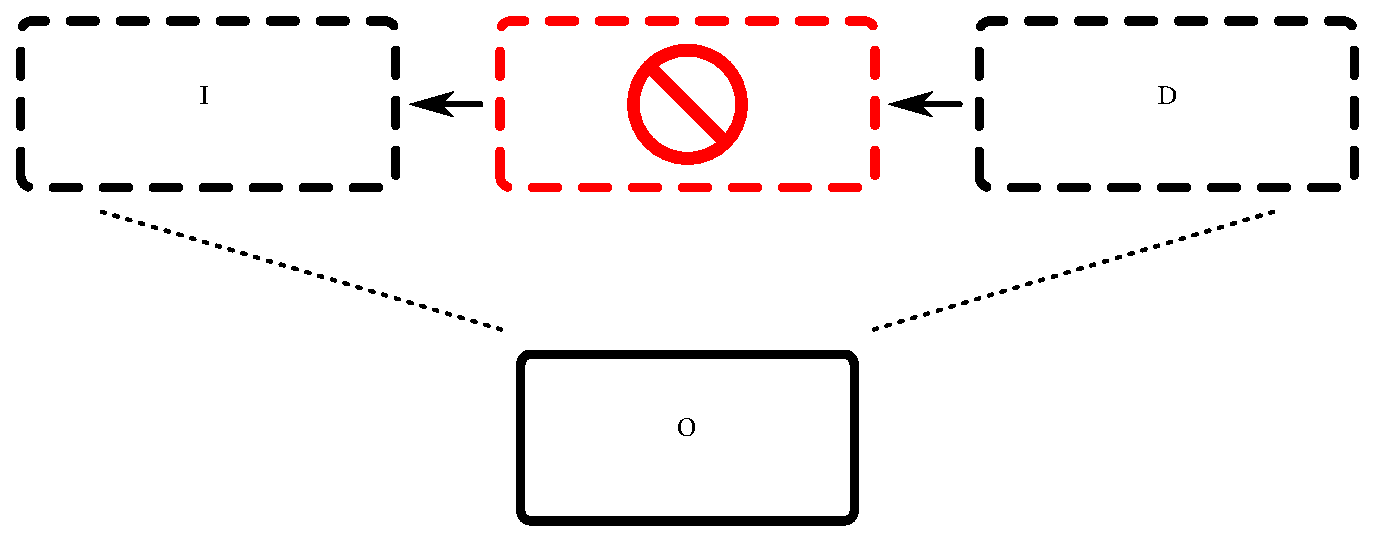
\epsfig{file=Figures/output,width=12.075cm}
\end{psfrags}
\end{center}
\caption{Components of the output block.}
\label{figure:BlockOutput}
\end{figure}

At the output of the system, the data must be transformed back into a format that is acceptable to the end-user.
The received message must be decompressed.
Note that for the destination to be able to recover the original data, it must understand the encoding scheme used by the sender.
In other words, the decoding method must be known at the receiver.
If the original signal is a continuous-time waveform, then an interpolator can be used to reconstruct the the waveform from its sample values.
The quantization block present at the input does not have a counterpart at the output.
This deficiency can be explained through the fact that quantization cannot be undone.
Information is lost whenever a continuous-space signal is discretized.
The level of \emph{distortion} associated with quantization can, however, be controlled by selecting an appropriate quantizer.


\subsection{The Transmitter-Receiver Pair}

A channel code is used at the transmitter to shield data sent over the channel against errors due to noise and interference.
This level of protection is achieved by adding redundancy to the information bits in a structured manner.
Audio CDs make use of a \emph{Reed-Solomon code} to protect the music from scratches and dust, whereas a low-latency \emph{convolutional code} is employed in cellphones to carry voice signals.
The second task of the transmission unit is to modulate the digital bit-stream onto an analog carrier prior to transmission.
The possible waveforms emitted by the transmitter are chosen from a finite number of symbols.
The transmitter must produce a signal that remains confined to its assigned spectral bandwidth.

\begin{figure}[htbp]
\begin{center}
\begin{psfrags}
\psfrag{T}[c]{Transmitter}
\psfrag{E}[c]{Encoder}
\psfrag{M}[c]{Modulation}
\epsfig{file=Figures/transmitter,width=7.7625cm}
\end{psfrags}
\end{center}
\caption{Components of a transmitter.}
\label{figure:BlockTransmitter}
\end{figure}

The message then propagates through the communication channel.
This is the physical medium that bridges the gap between the transmitter and the receiver.
In most applications, the channel acts as to transfer the data to a different place.
However, in hard disk drives and CDs, the information may be stored locally simply to be accessible at a later time.
Most communication channels cause signal degradation.
The message  may be subject to attenuation, interference and noise corruption.
The communication channel may be unreliable; and its environment, hard to characterize.
Recovering the original data from a set of measurements available at the receiver is one of the many challenges of digital communication systems.

\begin{figure}[htbp]
\begin{center}
\begin{psfrags}
\psfrag{R}[c]{Receiver}
\psfrag{M}[c]{Demodulation}
\psfrag{D}[c]{Decoder}
\epsfig{file=Figures/receiver,width=7.7625cm}
\end{psfrags}
\end{center}
\caption{Components of a receiver.}
\label{figure:BlockReceiver}
\end{figure}

The receiver is tasked with extracting the original symbols from noisy measurements.
The first step consists in producing estimates as to which symbols were sent by the transmitter over the channel.
This procedure is termed \emph{demodulation}.
These symbols estimates are then translated back into information bits by the decoder.
Redundancy is removed from the data, and the original format of the information bits is restored.
If the channel conditions are harsh and the local measurement too noisy, then this process fails and the corresponding data is lost.
Scratching a CD repetitively will illustrate this point well.
After substantial disc abuse, a player is not longer able to recreate the music.


\section{Common Channels}

Various communication channels can provide a connection between a transmitter and a receiver.
Common wireline channels include coaxial cables, ethernet cables, and twisted-pair wires.
Optical fiber offers a high-capacity solution for heavy applications.
Finally, wireless electromagnetic channels are popular for their convenience and broadcast capabilities.


\section{Sample Applications}

Digital communication occupies a central role in almost every aspect of contemporary life.
Most businesses rely on networked computers and the Internet for day-to-day operations, and digital technologies play a central role in the entertainment industry today.
Below, we provide a few examples of digital communication systems that you may be familiar with.

\paragraph{Cable Modem:}
A cable modem enables point-to-point communication over the cable television infrastructure.
They are primarily employed to deliver broadband Internet access, taking advantage of unused bandwidth on a cable television network.
With the advent of Voice over IP telephony, cable modems can also be used to provide telephone service.

\paragraph{Wi-Fi Technology:}
Wi-Fi is a global set of standards that allows wireless inter-networking.
In particular, it includes the IEEE 802.11 protocol suite (e.g., 802.11b, 802.11g, and 802.11n).
Wireless access points, also called \emph{hotspots}, often provide users with access the Internet.
Wi-Fi products can be used as an enabling technology for \emph{mesh networks}, which offer connectivity to large urban communities.

\paragraph{Bluetooth:}
Bluetooth is a wireless protocol designed for short-range communication, and it is used primarily to create personal area networks.
Bluetooth provides a means to exchange information between such devices such as mobile phones, personal computers, digital cameras, and a myriad of accessories.

\paragraph{Hard Disk Drive:}
A hard disk drive is a non-volatile storage device that stores digitally encoded data on rapidly rotating platters with magnetic surfaces.
Today, hard drives can be found in computers, digital audio players, personal digital assistants, game consoles and other embedded computing devices.
Data on a hard disk drive is recorded by magnetizing ferromagnetic material directionally, and is read back by detection the magnetization of the material.

\paragraph{Compact Disc:}
The compact disc (CD) is an optical disc used to store digital data, and remains one of the popular playback media for commercial audio recordings.
A standard compact disc can store approximately 650 Megabytes of data.
In a recordable compact disc (CD-R), a photosensitive dye is used.
The write laser of a CD recorder changes the color of the dye to allow a standard CD player to read the data, just as it would with a standard stamped disc.
A re-recordable disc medium (CD-RW) uses a metallic alloy instead of a dye.
The write laser in this case is used to heat and alter the properties of the alloy, and hence change its reflectivity.
A CD-RW does not possess as great a difference in reflectivity as a stamped compact disc, and so many earlier audio players cannot read CD-RW discs, although most later CD audio players and stand-alone DVD players can. 


